\section{Empirical Study}
\label{sec:ex}
We evaluated the performance of {\methodName} in comparison with the Rep-based Anonymization (RA) and the Casting-based Anonymization (CA) methods.

Recall that the RA method first extracts a single representative deterministic instance 
via algorithms proposed by Parchas~{\etal} in~\cite{Parchas_Gullo_Papadias_Bonchi_2014}.
Then, RA utilizes the deterministic graph anonymization method~\cite{Boldi_Injecting_2012} to produce the sanitized output.
While, the CA method first casts the given uncertain graph into a weighted deterministic graph.
Then, CA utilizes the weighted graph anonymization method, proposed by Sudipto~{\etal}~\cite{Das_Anonymizing_2010} to generate the corresponding sanitized output. 
Finally, it re-casts the output to the probabilistic version.
\subsection{Experiment Settings}

% \begin{table}[t]
%     \centering
%         \caption{Characteristics of datasets and privacy parameters}
%     \scalebox{0.75}{
%         \begin{tabular}{l|c|c|c|c||c}
%         \hline 
%         \textbf{Name} & \textbf{Content}  & \textbf{Nodes}    & \textbf{Edges}    &\textbf{Edge Prob}     & \textbf{$\epsilon$}\\
%         \hline  
%         \textrm{PPI} & \footnotesize{Protein-protein Interaction}  &12K       &397K       & 0.29         &$10^{-2}$\\
%         \textrm{BK}  & \footnotesize{Location-based OSN}    &58K       &214K       &0.29          &$10^{-3}$ \\
%         \textrm{DBLP}& \footnotesize{Co-authorship Network} & 824K      &5M         & 0.46         & $10^{-4}$\\
%         \hline
%         \end{tabular}
%      }
%         \label{tab:dataset}
%     \vspace{-10pt}
% \end{table}

\begin{table}[t]
    \centering
        \caption{Characteristics of datasets and privacy parameters}
    \scalebox{0.85}{
        \begin{tabular}{|l|c|c|c||c|}
        \hline 
        \textbf{Name} & \textbf{Content}  & \textbf{Nodes}    & \textbf{Edges}  & \textbf{$\epsilon$} \\
        \hline 
        \hline  
        \textrm{PPI} & \footnotesize{Protein-protein Interaction}  &12K       &397K        &$10^{-2}$\\
        \textrm{BK}  & \footnotesize{Location-based OSN}    &58K       &214K        &$10^{-3}$ \\
        \textrm{DBLP}& \footnotesize{Co-authorship Network} & 824K      &5M         & $10^{-4}$\\
        \hline
        \end{tabular}
     }
        \label{tab:dataset}
    \vspace{-10pt}
\end{table}

\textbf{Datasets}~~We test them on three uncertain graphs: PPI, BrightKite (BK) and DBLP as described in Table \ref{tab:dataset}. They have been widely used in the study of uncertain graphs~\cite{Zhao_Detecting_2014,Potamias_K_2010,Jin_Distance_2011}. 

\begin{itemize}
	\item{PPI is a dataset of protein-protein interactions, provided by Disease Module Identification DREAM Challenge. The probability of any edge corresponds to the confidence that the interaction actually exists, which is obtained through biological experiments.}
	\item{Brightkite is a location-based social network. In this dataset, each node represent a user. The probability of any edge corresponds to the chance that two users visit each other.}
	\item{DBLP is a dataset of scientific publications and authors. Each node represent an author. Two authors are connected by an edge if they have co-authored in a project. The uncertainty on the edge denotes the likelihood that the two authors will collaborate in a new project.}
\end{itemize}
% Answer the question why use these dataset 
DBLP dataset only has a few probability values, while probability values of Brightkite  are generally very small. The PPI dataset has a more uniform probability distribution. We also present their degree distributions of “unique” nodes (with high degree and obfuscation level is smaller than 300). Observe that, all the three graphs have a heavy-tailed degree distribution. Namely, they are difficult to be obfuscated.

\textbf{Parameter Setting}~~We consider the obfuscation level $k$ in the range $[100,300]$, and possible tolerance values $\epsilon$ to explore their performance difference. 

\textbf{Statistics}~~For every obfuscated result, we sampled $N$ possible worlds to compute its statistics of interest. Note that it has been shown that 1000 possible worlds usually suffices to achieve accuracy converge.  Here, we report their discrepancy against the original one. The smaller discrepancy, the better uncertain graph data utility preserving.



\begin{figure*}[!htb]
    \centering
    \subfigure[PPI]{
    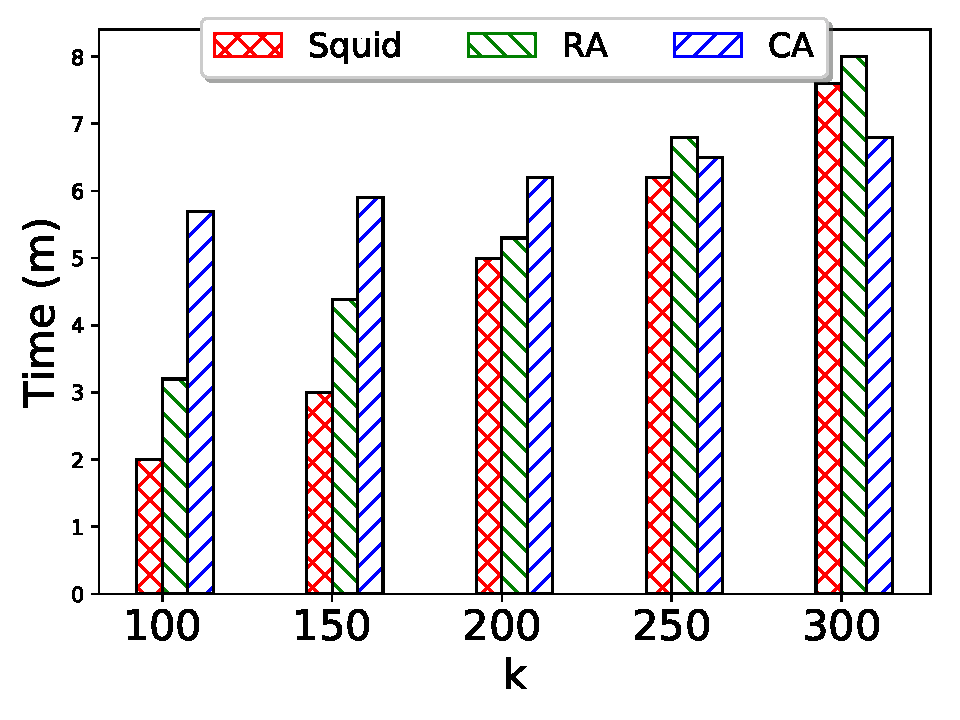
\includegraphics[width=.31\textwidth]{expResult/ppi_time.pdf}
    }
    \subfigure[BK]{
    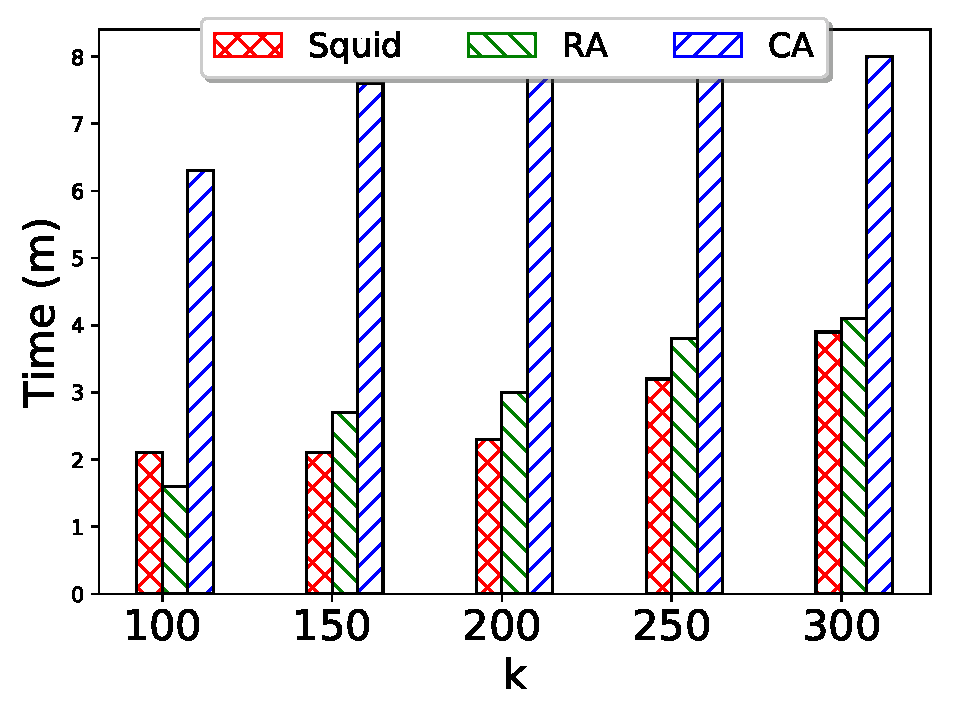
\includegraphics[width=.31\textwidth]{expResult/bk_time.pdf}
    }
    \subfigure[DBLP]{
    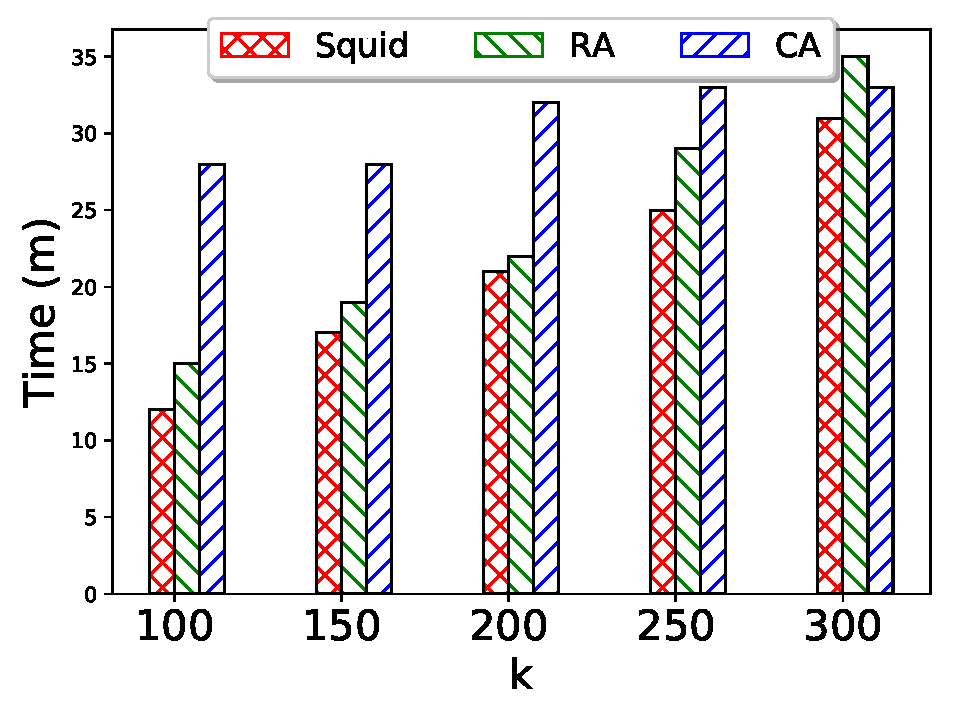
\includegraphics[width=.31\textwidth]{expResult/dblp_time.pdf}
    }
    \vspace{-5pt}
    \caption{Time efficiency of different anonymization methods on three real graphs.}
    \vspace{-5pt}
    \label{fig:time}
\end{figure*} 

\begin{figure*}[t]
    \centering
    \subfigure[PPI]{
    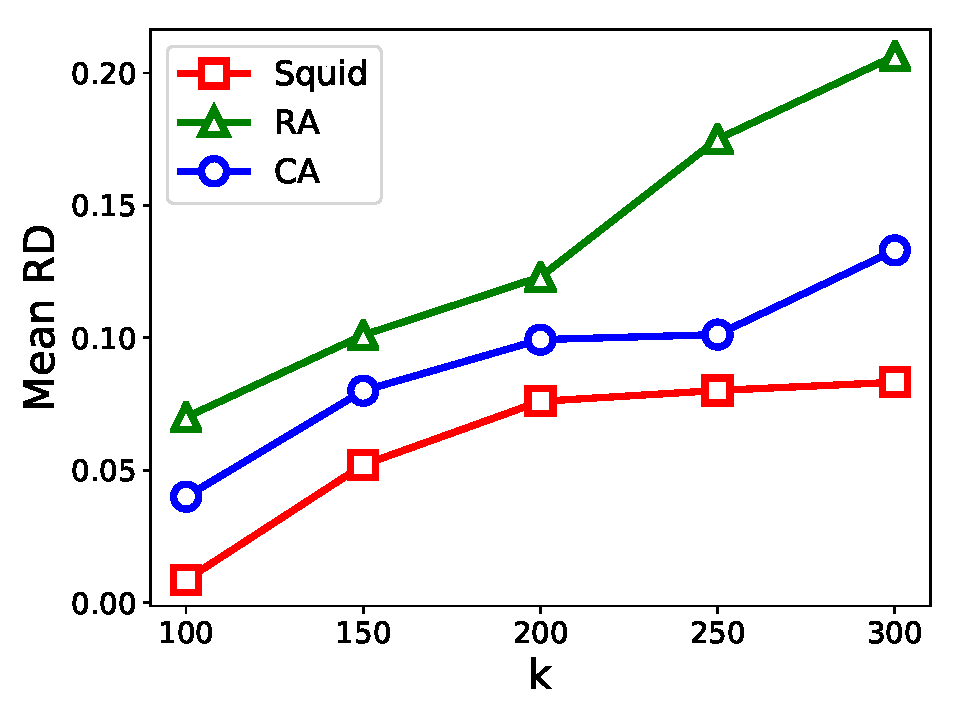
\includegraphics[width=.31\textwidth]{expResult/ppi_RD.pdf}
    }
    \subfigure[BK]{
    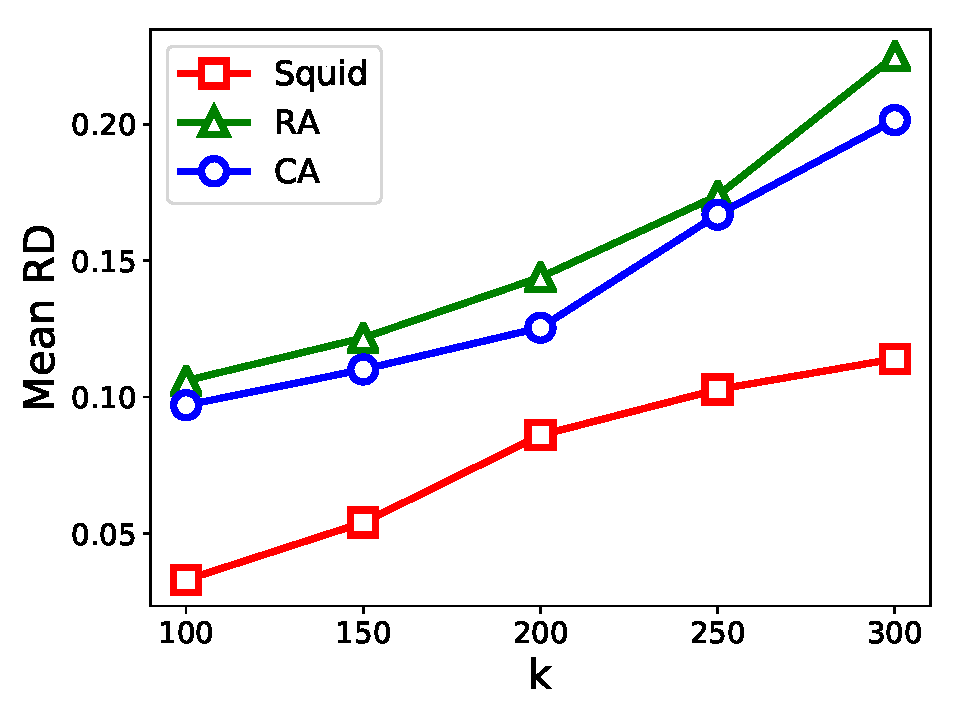
\includegraphics[width=.31\textwidth]{expResult/bk_RD.pdf}
    }
    \subfigure[DBLP]{
    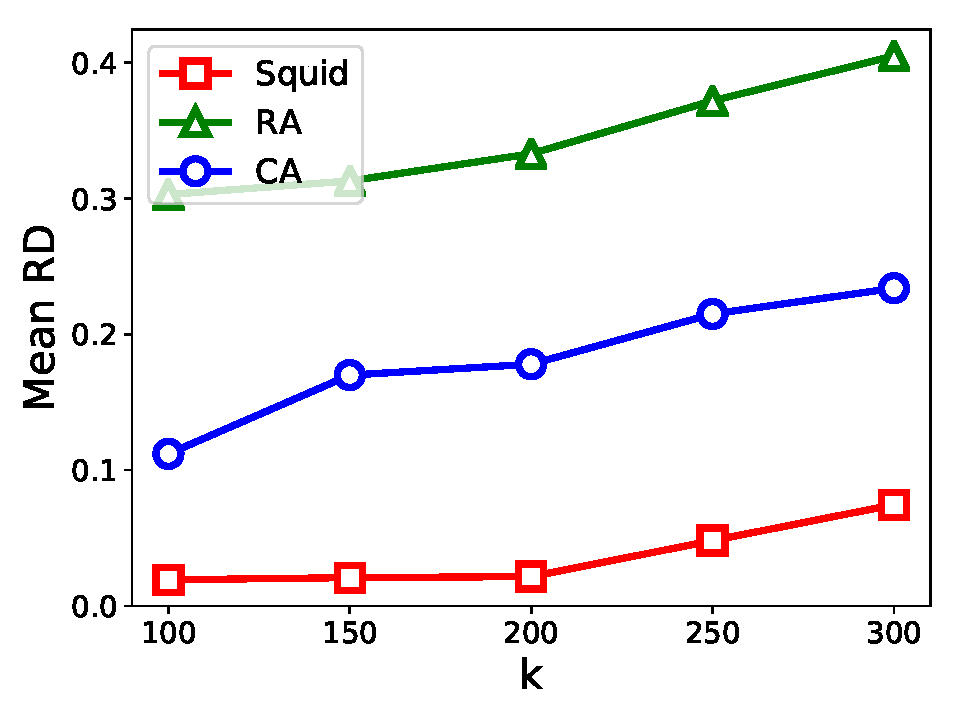
\includegraphics[width=.31\textwidth]{expResult/dblp_RD.pdf}
    }
    \vspace{-5pt}
    \caption{Reliability Discrepancy (RD) of sanitized output graphs of different anonymization methods against original graphs for various values of obfuscation parameter $k$. The smaller the discrepancy the more information of connectivity structure is preserved.}
    \label{fig:rd}
\end{figure*} 
\begin{figure*}[!htb]
    \centering
    \subfigure[PPI]{
    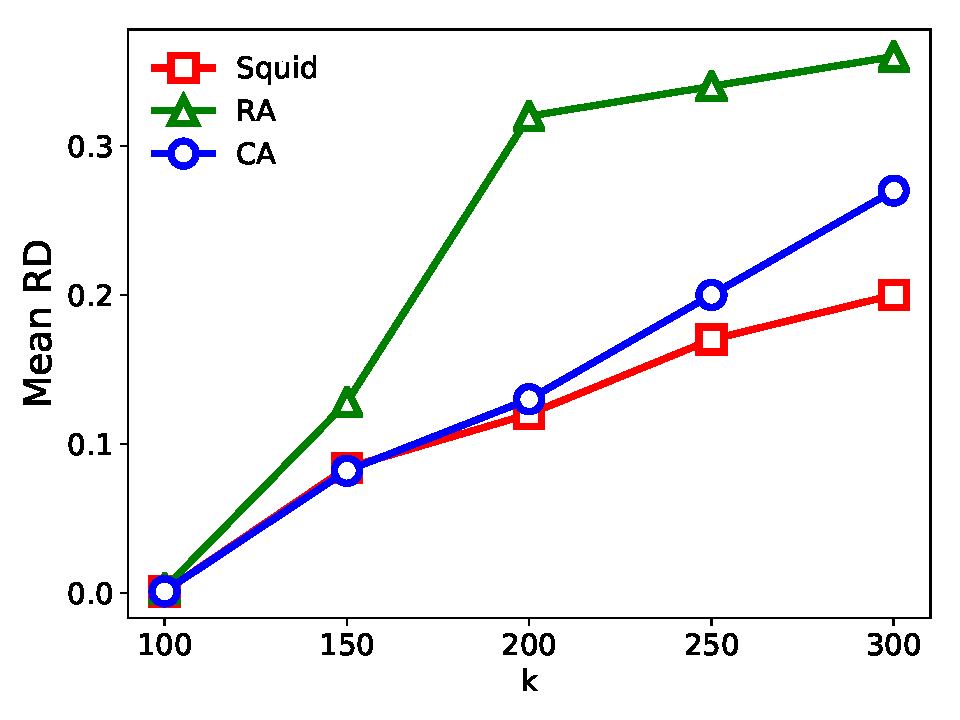
\includegraphics[width=.31\textwidth]{expResult/ppi_PathD.pdf}
    }
    \subfigure[BK]{
    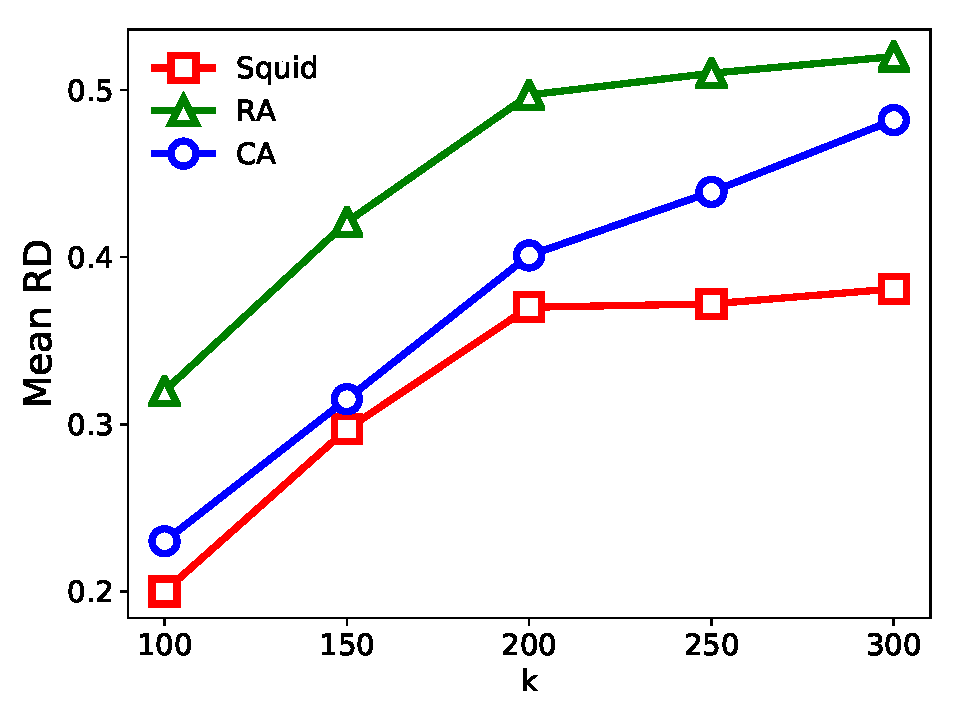
\includegraphics[width=.31\textwidth]{expResult/bk_PathD.pdf}
    }
    \subfigure[DBLP]{
    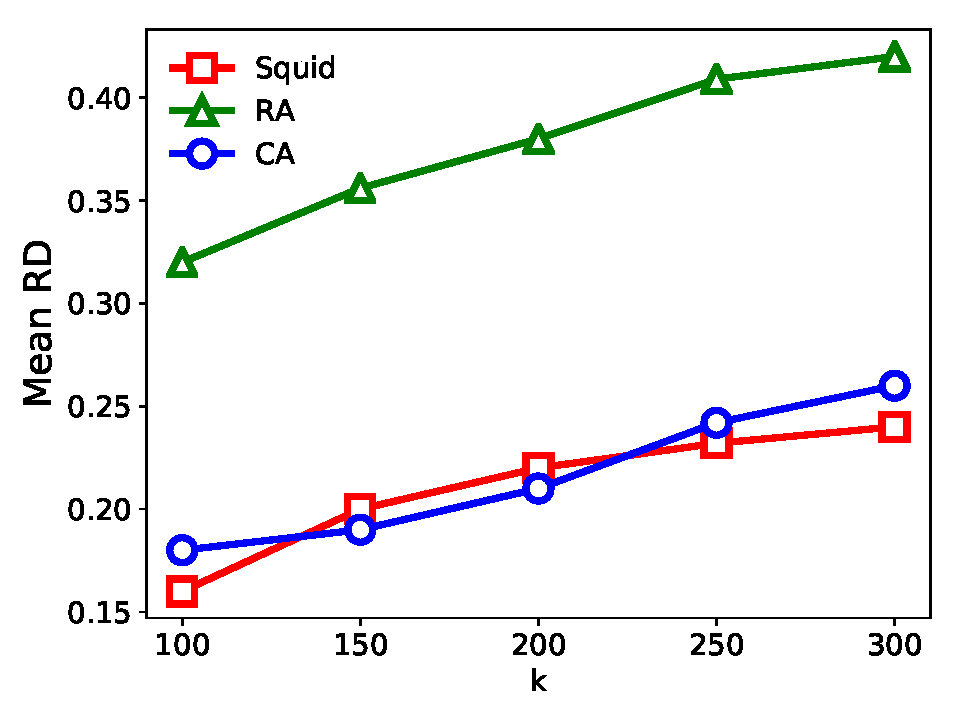
\includegraphics[width=.31\textwidth]{expResult/dblp_PathD.pdf}
    }
    \vspace{-5pt}
    \caption{Relative error of Shortest Path Distance (SPD) of sanitized output graphs of different anonymization methods against original graphs for various values of obfuscation parameter $k$.}
    \label{fig:rd}
\end{figure*} 

\vspace{-6pt}
\subsection{Results on time efficiency}
These anonymization algorithms were implemented in C++ and run on Intel Core i7 CPU, 2 GHZ, 6MB cache size. We plot their running times on on tested datasets (PPI, BK, DBLP) in Figure~\ref{fig:time}. For larger values for anonymity level $k$, all the methods take more time to find the sanitized solutions. It is because the increased efforts (more noises \& more modified edges) needed to achieve the higher anonymity level (larger values of $k$). 
In comparison, our {\methodName} achieves the comparable efficiency with RA and CA methods.  

As excepted, the time efficiency of our {\methodName} is close to RA, better than CA.
{\methodName} and RA use the randomized search strategy to identify sanitized uncertain solutions using the given standard deviation $\sigma$, while {\methodName} takes a connectivity model instead of degree sequence adopted in RA. 
The computation generalized uniqueness and relevance metrics can be finished off-line.
As we mentioned, multi-heuristics can co-boost the randomized search strategy in the quite straightforward way with little extra effort. 


\begin{figure*}[!htb]
    \centering
    \subfigure[PPI]{
    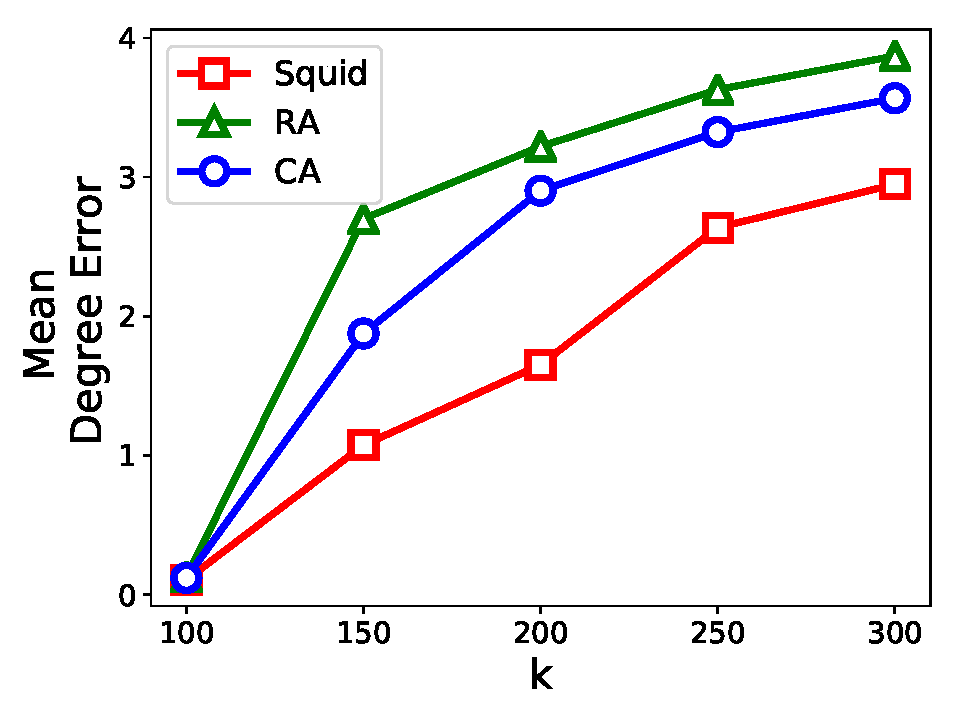
\includegraphics[width=.31\textwidth]{expResult/ppi_dd.pdf}
    }
    \subfigure[BK]{
    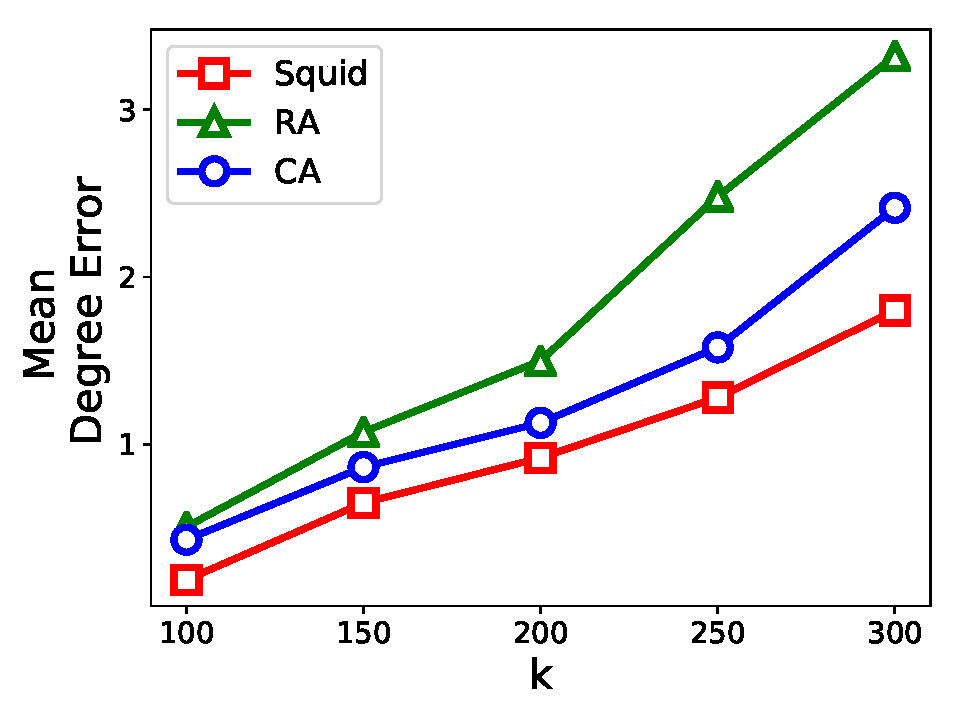
\includegraphics[width=.31\textwidth]{expResult/bk_dd.pdf}
    }
    \subfigure[DBLP]{
    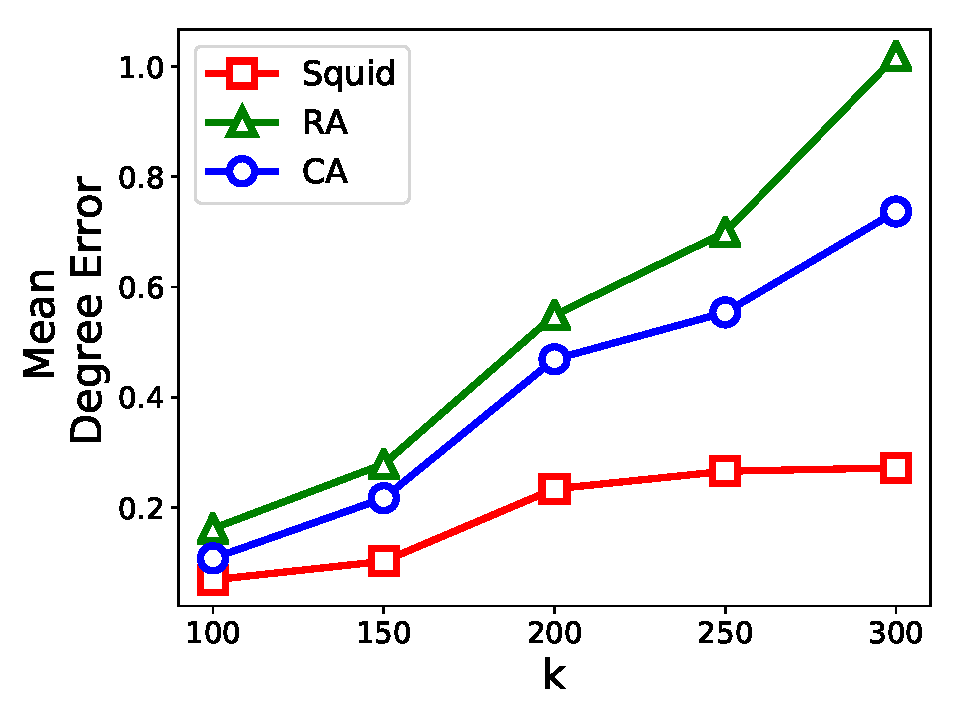
\includegraphics[width=.31\textwidth]{expResult/dblp_dd.pdf}
    }
    \vspace{-5pt}
    \caption{Degree error of sanitized uncertain graphs of different anonymization methods on three real graphs for various values of obfuscation parameter $k$. The smaller the degree error the more information of degree distribution is preserved.}
    \vspace{-5pt}
    \label{fig:dd}
\end{figure*} 
\subsection{Uncertain Graph Statistic Preserving}
In the set of experiment, we focus on evaluating their performance concerning statistic preserving. 
The evaluation includes two groups of graph statistics. 
The first group includes node separation statistics that quantify the interconnectivity and density of the overall graph.   
This group includes metrics such as Shortest Path Length~\footnote{In particular, we use Hyper ANF~\cite{Boldi_Rosa_Vigna_2011} to approximate shortest path-based statistics.},Reliability and Graph Diameter. 
The second group includes degree-based statistics such as Average  Node Degree and Degree Distribution.
These topological statistics that characterize how degrees are distributed among nodes. 
Our results are highly consistent across our pool of graph statistics.
For brevity, we report only Reliability, Shortest Path Length and Node Degree as their representatives. 

\textbf{Node Separation Statistic.} 
We plot the connectivity distortion introduced by anonymity process in Figure~\ref{fig:rd}.  
As expected, larger $k$ introduced more significant connectivity distortion, because more noise was added to achieve the desired level of anonymity.   
These observations are consistent across biological and social uncertain graphs.

There is a clear improvement of {\methodName} over CA and RA methods for the integration of possible world semantics and uncertain-aware search strategy. 
For example, in all the dataset ($k=300$), the reliability discrepancy introduced by {\methodName} is well below 0.1 whereas the ones added by CA is below 0.2. The reliability discrepancy introduced by RA on PPI, BK, DBLP is around 0.2, 0.2, 0.4 respectively. We also observe that as the size of graph increases (PPI $\rightarrow$ DBLP), the performance gap becomes larger and larger.

Note that CA and RA schemes deteriorate data utility due to the disregarding the possible world semantics. 
For example, in the case, $k=100$ (weak privacy guarantee required little noise), CA and RA incur relatively large connectivity distortion. 
The representative extraction step of RA introduces noise and results in cumulative errors in the anonymization step. Consequently, sanitized results differ from the original ones. 
The CA scheme fails to reflect the connectivity of uncertain graph correctly. Therefore, it produces inferior results even with the focused anonymization strategy. 


\textbf{Degree-based Statistic.}~Figure~\ref{fig:dd} shows the error of Node Degree values on PPI, BK and DBLP compared to their sanitized outputs. 
The obfuscated output of {\methodName}, CA capture well Node Degree in all datasets; 
our method {\methodName} is consistently better.    
In the largest dataset DBLP, the degree error $0.2$ is much lower than $1.08$ imposed by the two-phase anonymization scheme (RA) in the same level of obfuscation ($k=300$).  
As with previous experiments, the performance gap increases as the graph size increases.

\textbf{Summary.} 
Our experimental results show that sanitized outputs generated by {\methodName} exhibit structural features close to those of their original uncertain graphs. 
Results show that we are able to effectively balance the utility and privacy in the probabilistic graph context.
The result is encouraging because we can eliminate the noise by moving from the reliability model to a more accurate graph model incorporating with the possible world semantics.
\subsection{Uncertain Graph Application Measures}
\begin{figure}[!htb]
    \centering
    \subfigure[PPI]{
    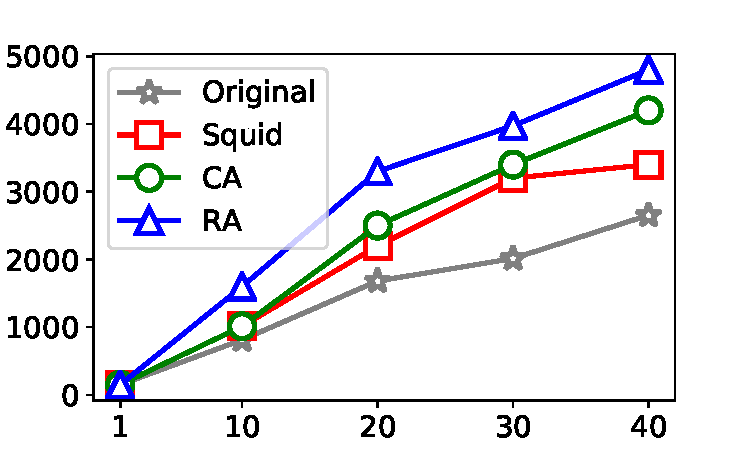
\includegraphics[height=4cm]{expResult/ppi_IM.pdf}
    }
    \subfigure[BK]{
    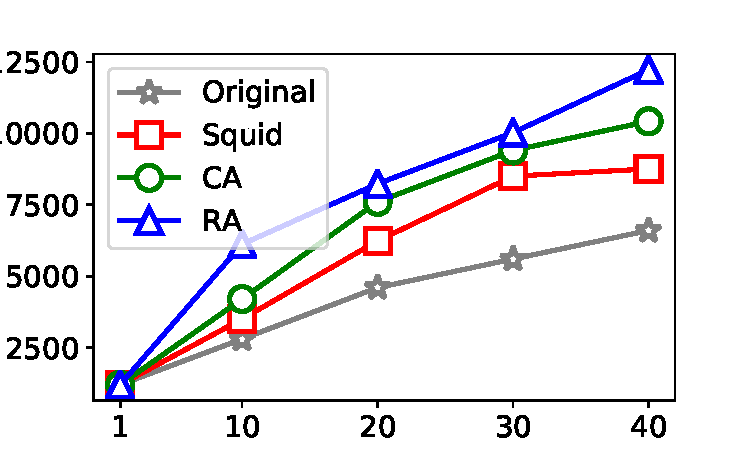
\includegraphics[height=4cm]{expResult/bk_IM.pdf}
    }
    \caption{ Results of the influence maximization algorithm on PPI and BK datasets, compared to sanitized outputs where $k$=100.}
    \vspace{-15pt}
    \label{fig:IM}
\end{figure} 
For a sanitized graph to be meaningful for research use, it should produce 
the close results as the original graph in the application-level settings. 
Influence Maximization is known as essential techniques with advertisement and public relation campaigns.
It tries to locate users in the network who can most quickly spread information through the network. 
Usually, related algorithms start with identifying the nodes which can maximize influence and model the spread of influence through network how many users has ultimately reached.  
Motivated by these facts, we compare the result of influence maximization on sanitized outputs and original graphs. 
In general, it enables us to quantify the trade-off between application utility and privacy protection. 

\textbf{Methodology.}~We used the sampling method to get the expectation value of influence. For each sampled graph, we adopt the degree discount method (a heuristic-based method with light computation) to find the most influential nodes (seeds) on a deterministic graph. Starting from those seeds, we run the weighted cascade influence dissemination model to determine the number of reached users in the network. 

For the limit of computation resource (memory overhead), we only perform the set of experiment over PPI and BK datasets. We report the expected number of reached nodes when the number of initial seeds in Figure~\ref{fig:IM}. 
There are clear and visible trends across PPI and BK datasets. 
Graphs with privacy protection diverge from the results of original graphs.
We can see that {\methodName} produces closer results with the identical privacy protection, comparison to CA and RA methods. 
Overall, our experimental assessment on influence maximization applications confirms our intuition: by incorporating the possible world semantics into the core of anonymization such as edge selection and uncertainty injecting, one can achieve the same desired level of anonymity with a smaller impact in the uncertain graph utility.  
